% SDC 2026 Midterm01 -- Localization report
% Build (XeLaTeX + xeCJK; run twice for references):
%   cd midterm01/report && xelatex localization_report.tex && xelatex localization_report.tex
% Fonts: kaiu.ttf (DFKai-SB) must be installed on the machine that compiles.
\documentclass[11pt, a4paper]{article}

% --- 必要套件 ---
\usepackage[margin=2.5cm]{geometry}
\usepackage{graphicx}
\usepackage{xcolor}
\usepackage{listings}
\usepackage{caption}
\usepackage{float}
\usepackage{amsmath}
\usepackage{amssymb}
\usepackage{booktabs}
\usepackage{xeCJK}
\usepackage{hyperref}
% 本報告額外使用
\usepackage{tabularx}
\usepackage{array}
\usepackage{enumitem}

\setCJKmainfont[AutoFakeBold=2.5]{kaiu.ttf}
\setCJKsansfont[AutoFakeBold=2.5]{kaiu.ttf}


% --- 設定圖片標題文字置中集中，不左右分散 ---
\captionsetup[figure]{justification=centering}

\setlist{itemsep=2pt,topsep=4pt,parsep=0pt}
\renewcommand{\arraystretch}{1.15}

% inline code; \detokenize keeps underscores and braces literal
\newcommand{\code}[1]{\texttt{\detokenize{#1}}}
\newcommand{\dg}{$^{\circ}$}
\newcolumntype{Y}{>{\raggedright\arraybackslash}X}

% --- 程式碼區塊樣式設定 ---
\definecolor{codegreen}{rgb}{0,0.6,0}
\definecolor{codegray}{rgb}{0.5,0.5,0.5}
\definecolor{codepurple}{rgb}{0.58,0,0.82}
\definecolor{backcolour}{rgb}{0.96,0.96,0.96}

\lstdefinestyle{bashstyle}{
    backgroundcolor=\color{backcolour},
    commentstyle=\color{codegreen},
    keywordstyle=\color{blue},
    numberstyle=\tiny\color{codegray},
    stringstyle=\color{codepurple},
    basicstyle=\ttfamily\footnotesize,
    breakatwhitespace=false,
    breaklines=true,
    captionpos=b,
    keepspaces=true,
    numbers=none,
    showspaces=false,
    showstringspaces=false,
    showtabs=false,
    tabsize=2,
    frame=single,
    rulecolor=\color{black!20}
}

\lstdefinestyle{cppstyle}{
    backgroundcolor=\color{backcolour},
    commentstyle=\color{codegreen},
    keywordstyle=\color{blue},
    numberstyle=\tiny\color{codegray},
    stringstyle=\color{codepurple},
    basicstyle=\ttfamily\footnotesize,
    breakatwhitespace=false,
    breaklines=true,
    captionpos=b,
    keepspaces=true,
    numbers=none,
    showspaces=false,
    showstringspaces=false,
    showtabs=false,
    tabsize=2,
    frame=single,
    rulecolor=\color{black!20},
    language=C++
}

\lstset{style=bashstyle}

\title{SDC 2026 Midterm01 Localization 報告\\[2pt]
\large 影像點雲對 LiDAR 地圖的 Causal 定位}
\author{第 7 組\quad 王修呈（a151527）}
\date{2026 年 11 月}

\begin{document}
\maketitle

%--------------------------------------------------------------------
\begin{abstract}
本作業以 LoGeR 由前鏡頭影像產生的點雲（\code{raw_ply}）對預建的 LiDAR 地圖
（\code{map.pcd}）做 scan matching，估計每個影像幀的車輛位姿。影像點雲沒有絕對尺度、
縱向幾乎不可觀測，直接對地圖做 NDT 會在停等、起步與轉彎時失效。
本報告從這些問題出發，建立一條 \emph{causal} 的估計管線：以 IMU 驅動的 7 狀態 EKF 為主體，
NDT 多起點對齊的候選經軟加權融合後作為量測；並針對（A）縱向退化與單幀不穩、
（B）停等與起步的漂移、（C）第 0 幀初始位姿不可靠、（D）行駛中 yaw 的系統性偏差、
（E）缺乏全域錨定五類問題，分別提出對應的解法。
其中\textbf{第 0 幀初始位姿搜尋}與\textbf{地圖牆面方向先驗}、\textbf{地圖軌跡線航向量測}為本作業的原創設計。
三個 track 的 Kaggle 成績如表~\ref{tab:summary}：Track1/2 通過 baseline，Track3 的 private 分數通過 baseline。
\end{abstract}

\begin{table}[H]
\centering\small
\caption{三個 track 的正式版與 Kaggle 成績}\label{tab:summary}
\begin{tabularx}{\linewidth}{@{}llcccY@{}}
\toprule
Track & 權重 $r$ & 正式版 & Kaggle & Baseline & 結果\\
\midrule
Track1 & 0.3 & \code{gb} & \textbf{1.13} & 1.79 & 通過\\
Track2 & 0.3 & \code{g2b} & \textbf{0.77} & 1.92 & 通過\\
Track3 & 0.4 & \code{p5} & public \textbf{1.74}／private \textbf{1.36}
       & public 1.29／private 1.40 & public 未達；private 通過\\
\bottomrule
\end{tabularx}
\end{table}

%====================================================================
\section{問題與解法總覽}

\subsection{任務與輸入特性}
\begin{itemize}
  \item \textbf{輸入}：每幀約 15k--41k 點的 PLY（$x$ 前、$y$ 左、$z$ 上）、ASCII 地圖（約 57--60 M 點）、
        帶雜訊的 \code{init_guess.txt}、bag 內約 100~Hz 的 IMU；Track1/2 另有約 4~Hz 的 GNSS。
  \item \textbf{輸出}：每幀 $T_{\mathrm{map}\leftarrow\mathrm{body}}$，轉成 Kaggle 的 \code{idx,x,y,yaw}。
  \item \textbf{評分}：
        $E=\sqrt{\tfrac1N\sum\lVert\Delta p\rVert^2}+0.2\sqrt{\tfrac1N\sum\Delta\theta^2}$
        （$\Delta p$ 為公尺、$\Delta\theta$ 為度）；yaw 的 RMS 每度折合 0.2，5\dg{} 就是 1.0。
  \item \textbf{輸入的三個先天限制}：（1）點雲\textbf{沒有絕對尺度}（深度約 0.2--5 個單位）；
        （2）影像深度在前進方向上誤差大，\textbf{縱向幾乎不可觀測}；
        （3）點雲與地圖來自不同感測器，NDT 的最佳點本身很平坦。
\end{itemize}

\subsection{問題樹}
我們把開發過程中遇到的問題整理成表~\ref{tab:tree}。每個問題先說明現象與根因，再說明解法；
括號內標示該問題是在哪個 track 上首先觀察到的。

\begin{table}[H]
\centering\small
\caption{問題與解法對照（由上而下）}\label{tab:tree}
\begin{tabularx}{\linewidth}{@{}l>{\raggedright\arraybackslash}p{0.2\linewidth}>{\raggedright\arraybackslash}p{0.2\linewidth}Y@{}}
\toprule
 & 問題（觀察於） & 根因 & 解法\\
\midrule
A & 單幀 NDT 位置每幀跳動、縱向不穩（Track1） & 縱向退化；NDT 最佳點平坦
  & 多起點軟加權融合，候選分散度進量測協方差；IMU 預測的 EKF（第~\ref{sec:A} 節）\\
B & 停等時位置與 yaw 漂移、起步被誤判為靜止（Track3 紅燈、Track2 起步）
  & 靜止時沒有視差；小加速度起步被當成零偏
  & ZUPT 與靜止鎖定；加速度條件與偽量測（第~\ref{sec:B} 節）\\
C & 第 0 幀航向有數十度誤差（Track3、Track2）
  & \code{init_guess} 帶雜訊；靜止起步的單幀 NDT 對 yaw 沒有鑑別力
  & \textbf{初始位姿搜尋}、\textbf{牆面方向先驗}、YawBank（第~\ref{sec:C} 節）\\
D & 行駛中 yaw 有系統性偏差、轉彎過早（Track3）
  & NDT 的 yaw 被單側結構拉偏
  & \textbf{地圖軌跡線航向量測}（第~\ref{sec:D} 節）\\
E & 位置與 yaw 缺乏全域錨定（Track1/2）
  & 純相對估計，誤差累積
  & 融入官方提供的 GNSS 先驗（第~\ref{sec:E} 節）\\
\bottomrule
\end{tabularx}
\end{table}

\subsection{系統架構}
\begin{figure}[H]
\centering
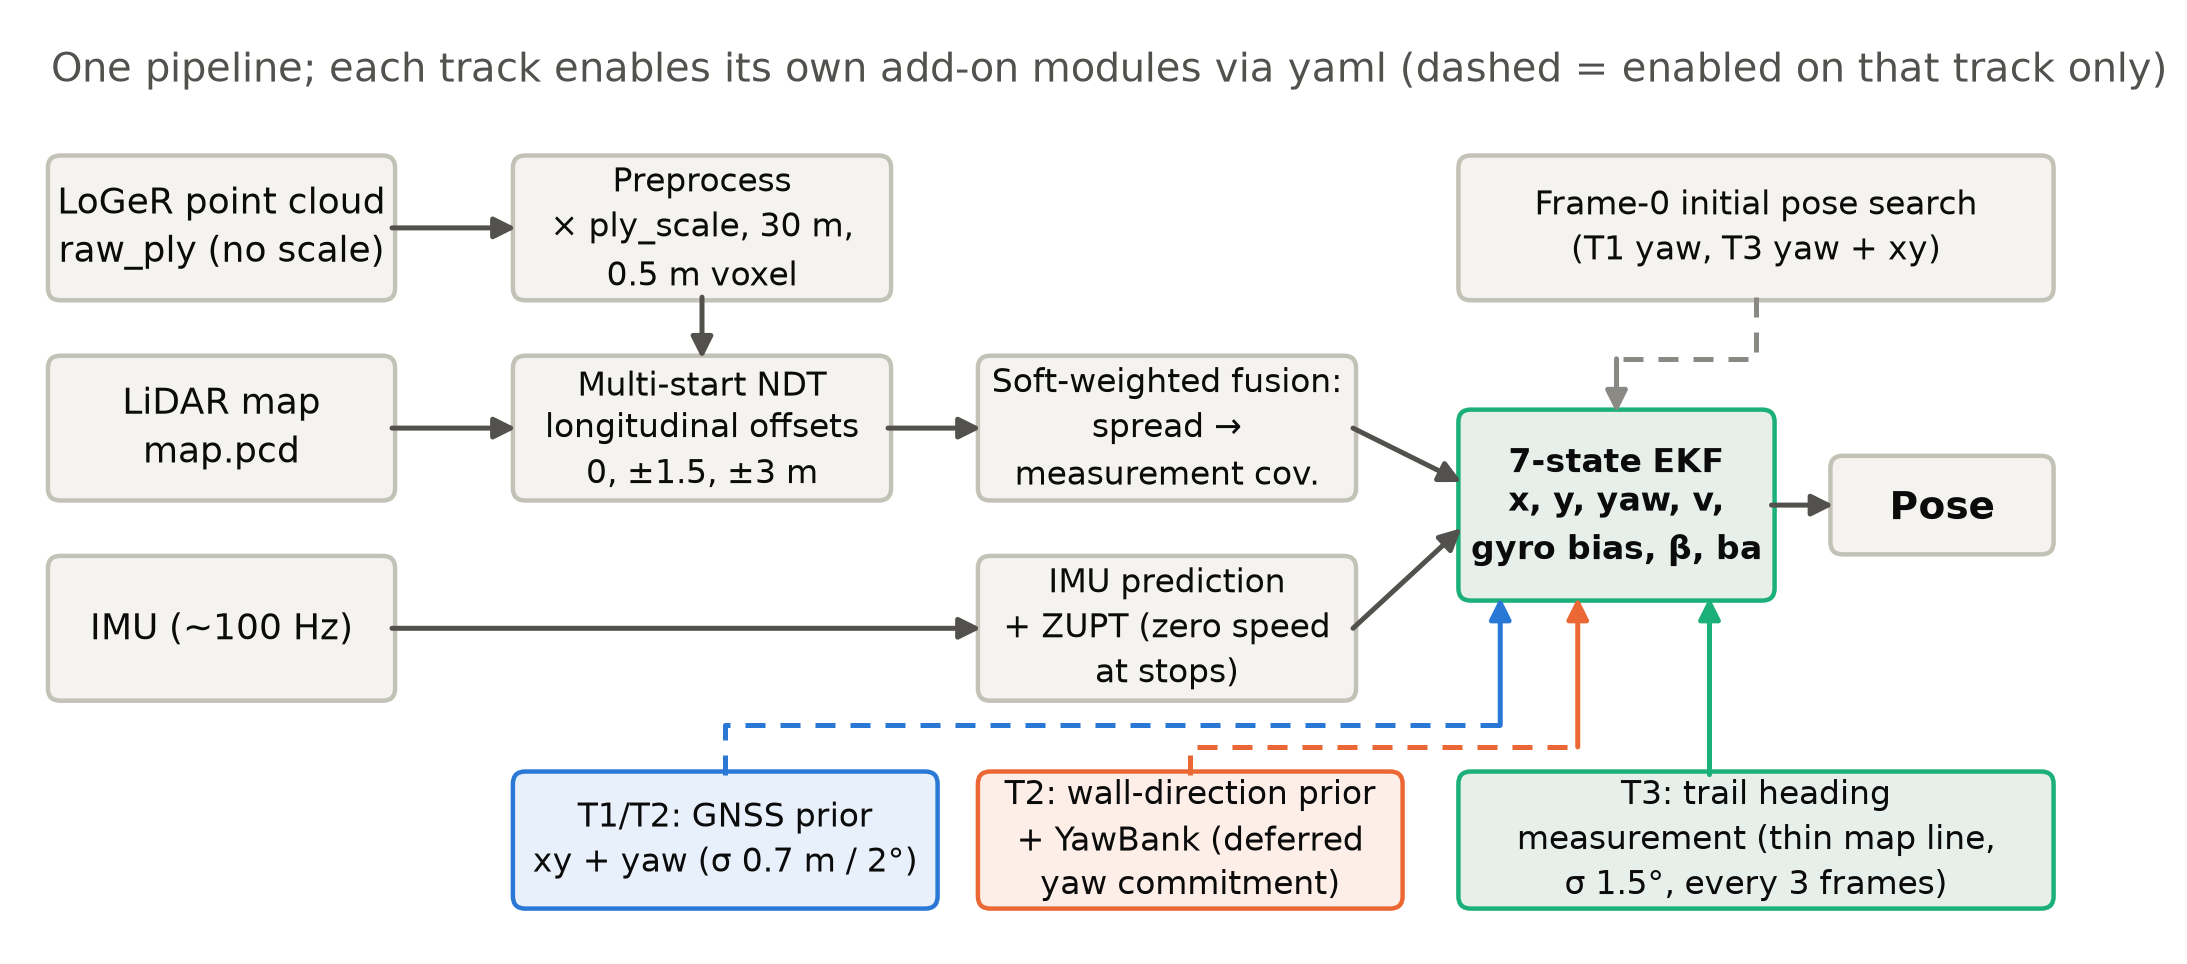
\includegraphics[width=\linewidth]{figures/m2_architecture.png}
\caption{整體管線。同一條管線，各 track 以 yaml 開啟自己的外加模組（虛線＝僅該 track 啟用）。}
\label{fig:arch}
\end{figure}

每一幀依序執行：IMU 預測 $\to$ 多起點 NDT 對齊與候選融合 $\to$ EKF 量測更新
$\to$（依 track）GNSS／軌跡線的航向與位置更新。第 0 幀額外執行初始位姿搜尋與牆面方向先驗。

\subsection{規則遵守}
\begin{itemize}
  \item \textbf{Causal}：第 $k$ 幀只用第 $0..k$ 幀的 PLY 與時間戳不晚於影格時間的 IMU／GNSS 樣本。
  \item \textbf{無後處理、無 leaderboard probing}：Kaggle 分數只用來比較方法與設定，沒有用來反推誤差再修正軌跡。
  \item \textbf{GNSS}：官方文件明文允許，僅用於 Track1/2（Track3 的 bag 沒有 GNSS）；
        Track2 地圖中意外遺留的 \code{tl}/\code{th} 欄位完全沒有使用。
  \item \textbf{可重現}：每個 track 有一份完整 yaml；以純 yaml 全長重跑的結果與正式結果檔\textbf{逐位元相同}。
\end{itemize}

%====================================================================
\section{問題 A：縱向退化與單幀 NDT 不穩}\label{sec:A}

\subsection{前處理與尺度}
點雲先乘上各 track 的尺度（Track1/2/3 為 8.5/8.7/7.5），保留水平 30~m 內的點，再以 0.5~m 體素降採樣
（遠處的單目深度誤差大）。地圖離線降採樣成 1~m 體素的 binary 快取，執行時只截取車輛周圍
水平 $\pm50$~m、垂直 $\pm15$~m 的子地圖，車輛移動超過 10~m 才重新截取。

尺度未知是第一個問題。我們以固定位姿掃描尺度並比較對齊分數，行駛段的最佳尺度穩定
（Track3 為 7.5）；停車段因為沒有視差，最佳尺度會偏離，但此時位置已被 ZUPT 鎖住，影響有限。
我們也嘗試過「線上估計尺度」（每 3 幀以 5 個等比候選尺度比較 NDT fitness），但 fitness 較好的尺度會吸收平移誤差
（尺度與平移耦合），Track1 本地 $E$ 反而由 1.73 變差為 2.24，因此放棄，改用各 track 固定的尺度。

\subsection{現象與根因}
若每幀對多個起點做 NDT、再取 probability 最大的候選當量測，量測會在不同模式之間翻轉，每幀跳動約 1~m。逐幀檢查發現：
\begin{itemize}
  \item 影像點雲的縱向分散很大：以不同縱向起點對同一幀對齊，結果的縱向分散中位數為 1.13~m；
        NDT 單幀只能把誤差往真值方向拉約 19\%。
  \item NDT 的誤差在時間上相關（貼著預測走），因此只靠調整雜訊參數無法同時既「誠實」又更準。
  \item 取 probability 最大者（argmax）會在不同模式之間翻轉，濾波器完全不知道這一幀其實是曖昧的
        （本地 $E=3.88$）。
\end{itemize}
因此我們的設計原則是：\textbf{不要相信單一個 NDT 答案，而是把「這一幀有多曖昧」量化後交給濾波器}。

\subsection{多起點 NDT}
以 EKF 預測位姿為中心，沿預測航向取縱向偏移 $0,\ \pm1.5,\ \pm3$~m 共 5 個起點，各自執行一次 NDT
（PCL 的 NDT，解析度 3~m、步長 0.2、收斂門檻 0.01、最多 35 次迭代）。每個收斂的結果稱為一個\textbf{候選}，
帶有位姿 $T_i$ 與 NDT 的 transformation probability $p_i$。
起點只沿縱向展開，因為縱向正是最不確定的方向；橫向與 yaw 由 NDT 自己收斂。
如果所有候選都落在同一點，表示這一幀的答案很確定；若候選沿縱向散開，則表示縱向曖昧。

\subsection{候選軟加權融合}
令預測位姿的航向為 $\hat\psi$，第 $i$ 個候選相對預測的偏移在航向座標下分解為縱向 $o_i^{\mathrm{lon}}$、
橫向 $o_i^{\mathrm{lat}}$ 與 yaw 差 $o_i^{\psi}$。候選權重為
\begin{equation}
w_i\ \propto\ \left(\frac{p_i}{p_{\max}}\right)^{\kappa}
\exp\!\left[-\frac12\left(\frac{(o_i^{\mathrm{lon}})^2}{\sigma_{\mathrm{lon}}^2}
+\frac{(o_i^{\mathrm{lat}})^2}{\sigma_{\mathrm{lat}}^2}
+\frac{(o_i^{\psi})^2}{\sigma_{\psi}^2}\right)\right],\qquad \sum_i w_i=1,
\end{equation}
其中 $\kappa=4$（越大越接近 argmax），$(\sigma_{\mathrm{lon}},\sigma_{\mathrm{lat}},\sigma_{\psi})=(2~\text{m},\,1~\text{m},\,5^{\circ})$。
前一項偏好 probability 高的候選；後一項是以預測為中心的高斯先驗，避免被系統性偏後的候選拉走。
若所有權重都被先驗壓到 0（候選全離預測很遠），退回 probability 最大的候選。

融合後的量測為：位置（含 $z$）取加權平均 $\bar{\mathbf p}=\sum_i w_i\mathbf p_i$；
yaw 以最佳候選 $\psi_b$ 為參考取差值平均 $\bar\psi=\psi_b+\sum_i w_i\,\mathrm{wrap}(\psi_i-\psi_b)$
（避免角度繞圈）；roll/pitch 沿用最佳候選。同時計算候選相對加權平均的\textbf{分散度}
\begin{equation}
\Sigma_s=\sum_i w_i\,\boldsymbol\delta_i\boldsymbol\delta_i^{\top},\qquad
\boldsymbol\delta_i=\bigl(x_i-\bar x,\ y_i-\bar y,\ \mathrm{wrap}(\psi_i-\bar\psi)\bigr)^{\top},
\end{equation}
以及有效候選數 $n_{\mathrm{eff}}=1/\sum_i w_i^2$。$\Sigma_s$ 就是這一幀量測的\emph{經驗不確定度}：
候選一致則 $\Sigma_s\approx0$，縱向分歧則縱向方差變大。

\subsection{量測協方差與 EKF 更新}
EKF 的狀態為
$\mathbf x=[x,\ y,\ \psi,\ v,\ b_g,\ \beta,\ b_a]^{\top}$：位置、航向、速度、陀螺儀零偏、行進偏角、加速度零偏。
融合後的量測 $\mathbf z=(\bar x,\bar y,\bar\psi)$ 直接觀測前三個狀態（$H=[I_3\ 0]$）。量測協方差為
\begin{equation}
R_0=\mathrm{blkdiag}\!\Bigl(Q_{\beta}\,\mathrm{diag}(\sigma_{\mathrm{lon}}'^2,\ \sigma_{\mathrm{lat}}'^2)\,Q_{\beta}^{\top},\ \sigma_{\psi}'^2\Bigr)+g\,\Sigma_s,
\end{equation}
其中 $Q_\beta$ 是以航向 $\psi+\beta$ 構成的旋轉矩陣（把縱向給較大的方差，沿行進方向分解），
$(\sigma_{\mathrm{lon}}',\sigma_{\mathrm{lat}}',\sigma_{\psi}')=(1.1~\text{m},\,0.5~\text{m},\,4^{\circ})$，$g=1$。
也就是說，\textbf{基準雜訊給出「NDT 平均有多準」，候選分散度 $\Sigma_s$ 補上「這一幀有多曖昧」}。

為了避免單一個離群量測把狀態拉走，我們不丟棄量測，而是限制它的影響：令
$d^2=\boldsymbol\nu^{\top}S^{-1}\boldsymbol\nu$（$S=HPH^{\top}+R_0$、$\boldsymbol\nu$ 為創新），
當 $d^2$ 超過卡方門檻 11.34 時，把 $R$ 按比例放大 $d^2/11.34$。預測錯了仍可靠 $P$ 的成長慢慢拉回，
而不會像舊版「整幀被拒、速度被拉低、鎖死」那樣發散。更新用 Joseph 形式。
最後組回位姿：$x,y,\psi$ 取濾波結果，roll/pitch 與 $z$ 以增益 0.5 向 NDT 結果靠攏。

\subsection{IMU 預測}
預測用扣除零偏的陀螺儀積分更新航向，並以區間中點方向積分位置：
\begin{equation}
\psi_{k+1}=\psi_k+\Delta\psi_{\mathrm{gyro}}-b_g\Delta t,\quad
h=\psi_k+\tfrac12\Delta\psi+\beta,\quad
\begin{aligned}
x_{k+1}&=x_k+v\,\Delta t\cos h,\\ y_{k+1}&=y_k+v\,\Delta t\sin h,
\end{aligned}\quad
v_{k+1}=\mathrm{clip}\bigl(v+(a_{\mathrm{fwd}}-b_a)\Delta t,\ 0,\ v_{\max}\bigr),
\end{equation}
其中 $a_{\mathrm{fwd}}$ 是 IMU 姿態扣除重力後的前向加速度。縱向的速度完全由 IMU 提供，
NDT 縱向創新因為被 $\Sigma_s$ 降權，不會再把速度帶偏。

\subsection{考慮過但不採用的做法}
\begin{itemize}
  \item \textbf{G-ICP 取代 NDT}：收斂域較寬，但純追蹤時每幀跳 2--3~m，本地 $E$ 為 93--133。
  \item \textbf{累積多幀點雲}（$K=4/10$）：本地 $E=1.94/487$（發散），且耗時為 1.6--3.3 倍。
  \item \textbf{只調 $Q/R$ 的一致性校準}：$E=9.49/2.00/1.91$，不如軟加權（1.79）。
  \item \textbf{調整 NDT 參數與前處理}（解析度、最大距離、粗到細、去地面、離群點去除）：
        沒有任何一類在三個 track 同時提高收斂率與準度。NDT 的準度上限由點雲本身決定。
  \item \textbf{多相機點雲}：Track1 單幀準度與單相機打平，且對尺度更敏感。
\end{itemize}

%====================================================================
\section{問題 B：停等與起步的漂移與誤判}\label{sec:B}

\subsection{現象}
Track3 在約第 948--2179 幀停紅燈。停等時車輛靜止，連續幀之間沒有視差，NDT 的量測只剩雜訊；
這些雜訊經濾波器累積，造成位置與 yaw 持續漂移，陀螺儀零偏也被量測帶離真值（圖~\ref{fig:zupt}）。

\begin{figure}[H]
\centering
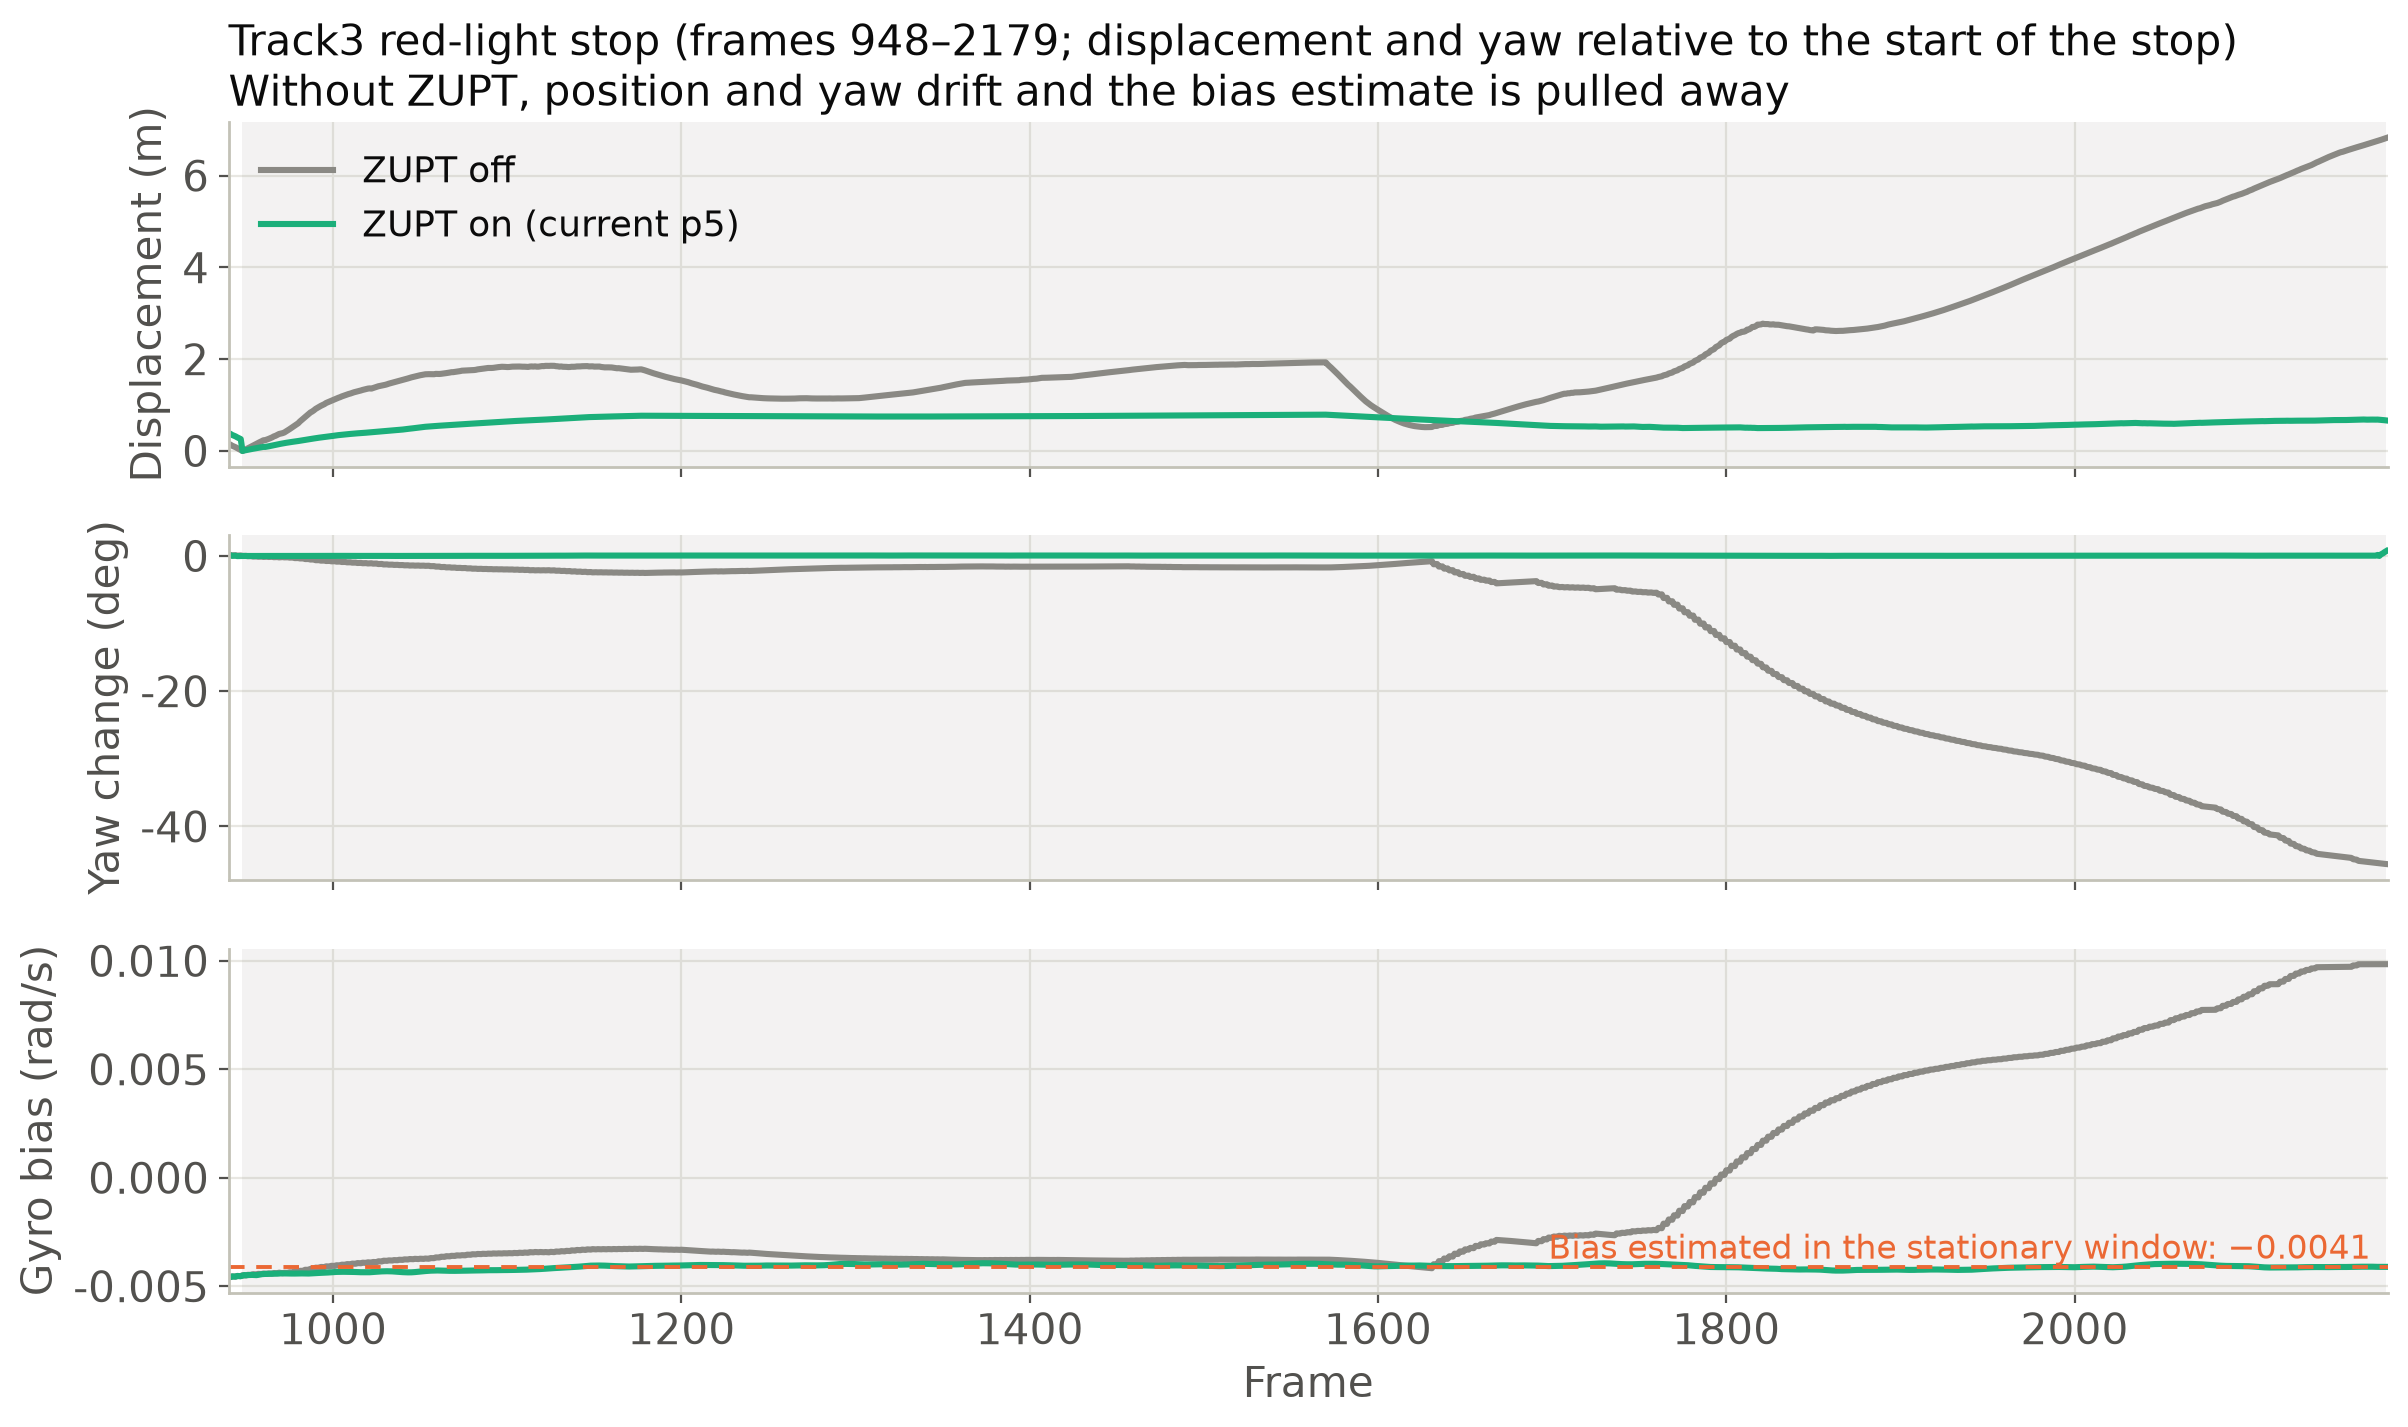
\includegraphics[width=0.92\linewidth]{figures/b2_zupt.png}
\caption{Track3 紅燈停等（第 948--2179 幀；位移與 yaw 皆相對停等起點）。
ZUPT 關（灰）時位移與 yaw 持續漂移、零偏被帶走；ZUPT 開（綠）時零偏穩定在靜止窗口估得的 $-0.0041$~rad/s。}
\label{fig:zupt}
\end{figure}

\subsection{解法：ZUPT 與靜止鎖定}
以 IMU 的滑動窗口（約 0.5~s）判定靜止：窗口內加速度與陀螺儀的標準差都小於門檻。靜止時：
\begin{enumerate}
  \item \textbf{零速更新}：速度偽量測為 0，陀螺儀均值當作零偏的觀測（並加上零偏先驗 $-0.004$）。
  \item \textbf{凍結 yaw}（\code{zupt_freeze_yaw}）：量測更新時，卡爾曼增益的\emph{整列} yaw 設為 0。
        只把 yaw 創新設為 0 是不夠的：位置創新會經由 yaw 與位置的交叉協方差把 yaw 轉走
        （我們實測在一次停等中被轉了 5.3\dg）。
  \item \textbf{位置鎖定}（\code{zupt_hold}）：位置不加過程雜訊；$z$ 與傾角不混入 NDT。
\end{enumerate}

\subsection{起步被誤判為靜止（Track2）}
Track2 以穩定的 0.33~m/s$^2$ 小加速度起步，此時窗口標準差很小，只看標準差會把起步誤判為靜止，
並把真實加速度當成零偏，導致速度損失、全長發散（本地 $E$ 218--670）。我們為 Track2 加上兩個條件：
\begin{itemize}
  \item 窗口加速度\emph{均值}必須接近目前的加速度零偏 $b_a$（偏離超過 0.08~m/s$^2$ 就不算靜止）；
  \item 靜止時對 $b_a$ 做偽量測（靜止時真實前向加速度為 0，量到的均值就是零偏）。
\end{itemize}
另外，把加速度零偏的過程雜訊由 0.01 降為 0.002（Track2/3），NDT 縱向創新就不再被當成 $b_a$，
解決了 Track3「太早轉彎」與轉彎後的橫縱向偏移（以 RViz 人工目視確認；差異出現在 private 區段）。

\subsection{證據}
表~\ref{tab:zupt} 為 Track3 第 948--2179 幀（約 1230 幀）的比較；ZUPT 關為 \code{p5} 設定加上
\code{-p zupt_enabled:=false}（run \code{zoff3}），ZUPT 開為現行 \code{p5}。零偏 $-0.0041$ 與靜止窗口估得的值一致。
Track3 的 Kaggle 由 3.98 降到 2.46，但該版同時改了 \code{ply_scale}（8.5$\to$7.5）與零偏先驗，
不能全歸功於 ZUPT。

\begin{table}[H]
\centering\small
\caption{Track3 停等段（第 948--2179 幀）ZUPT 開關比較}\label{tab:zupt}
\begin{tabular}{@{}lcccc@{}}
\toprule
 & 末端位移 & 停等段路徑長 & yaw 變化 & 第 2179 幀陀螺零偏\\
\midrule
ZUPT 關（\code{zoff3}） & 6.82~m & 18.01~m & $-45.6$\dg & $+0.0099$~rad/s\\
ZUPT 開（\code{p5}）    & 0.67~m & 1.84~m  & $+0.7$\dg  & $-0.0041$~rad/s\\
\bottomrule
\end{tabular}
\end{table}

\subsection{不採用：提高增益的 floor 補丁}
曾嘗試在靜止時提高量測增益（floor 0.6）來「讓量測多一點影響」：Track1 逐幀抖動變為 2.9 倍，
Track2 本地 $E$ 由 2.27 升到 16.96，Track3 靜止段路徑長由 3.9~m 升到 22.6~m，全部移除。
Track1 同一版（含搜 xy 格與 hold）的 Kaggle 由 1.56 退到 1.62，但本地 $E$ 卻由 1.79 變好為 1.7328——
這說明\textbf{本地 $E$ 會騙人}，必須同時看平滑度與 Kaggle。

%====================================================================
\section{問題 C：第 0 幀初始位姿不可靠}\label{sec:C}

\subsection{現象與根因}
\code{init_guess.txt} 帶有雜訊，尤其是航向。Track3 的 \code{init_guess} yaw 為 145.7\dg，而 IMU 內建姿態給出
167.2\dg，相差約 21.5\dg；Track2 的起點航向偏差約 15.2\dg。第 0 幀的初始航向錯誤會被後續估計繼承：
\begin{itemize}
  \item NDT 的收斂域有限，起點航向差二十多度時可能收斂到錯誤的局部最佳。
  \item 更棘手的是，\textbf{單幀 NDT 的 probability 對 yaw 是一個寬平台}（Track3 寬約 13\dg，Track1 更寬，
        Track2 近乎全平），單幀 argmax 只是雜訊。Track2 的車輛靜止起步，沒有視差，更是如此。
  \item 因果性不允許事後修正前面的輸出，而 yaw 每度折合 0.2：Track2 的 yaw 誤差幾乎全集中在第 0--300 幀
        （平均 $-13.8$\dg），只佔 9\% 的幀，卻貢獻幾乎整個 yaw RMS（約 4.2\dg）。
\end{itemize}
所以\textbf{起步時必須有好的初始 yaw}。我們設計了三個互補的機制：初始位姿搜尋、牆面方向先驗、YawBank。

\subsection{原創設計一：初始位姿搜尋}
\textbf{想法}：不相信 \code{init_guess} 的航向，而是在第 0 幀對多個航向假設各做一次 NDT，
讓地圖匹配決定初值。

\textbf{做法}：
\begin{enumerate}
  \item 搜尋中心有兩個：\code{init_guess} 的 yaw，以及 IMU 內建姿態的絕對航向
        （兩者獨立；IMU 姿態不累積積分誤差）。
  \item 以每個中心為準，在 $\pm30$\dg{} 內每 $5$\dg{} 取一個航向假設（每個中心 13 個）。
  \item 對每個航向假設，可再疊加縱向$\times$橫向的平移格（\code{init_search_xy_offsets}）：
        Track3 取 $\{0,\pm2\}\times\{0,\pm2\}$~m（9 格），共 $2\times13\times9=234$ 次 NDT；
        Track1 只搜 yaw（平移格 $\{0\}$），共 26 次；Track2 關閉（原因見下節）。
  \item 只改航向：在世界座標繞 $z$ 軸轉動，保留 \code{init_guess} 的 roll/pitch 與位置；
        對收斂的結果取 NDT probability 最大者，作為第 0 幀濾波器的初值，隨後仍以多起點 NDT 精修。
\end{enumerate}

\textbf{證據與限制}：
\begin{itemize}
  \item Track3：搜尋由 145.7\dg 選出 162.1\dg，與 IMU 姿態相差約 5\dg，落在地圖牆面方向範圍內
        （156.5--162.5\dg）；Kaggle 2.46$\to$2.01（該版同時加入「靜止時凍結 yaw」，兩者無法分開）。
  \item 由於 probability 在 yaw 上是寬平台，單幀 argmax 本身並不精確；它的作用是\textbf{把起點帶進收斂域}，
        後續幀由陀螺儀與 NDT 持續修正。我們也試過改用 fitness 當選擇準則，在 Track3 約 60 幀後兩者軌跡重合。
  \item \textbf{平移格在 Track1 有害}：它把起點移到 $(+1.8,+1.2)$~m，前 300 幀對 GNSS 的 RMS 由 1.49 增為 2.16，
        因為 Track1 的 \code{init_guess} 位置本來就準，而縱向是退化方向，NDT 會把起點挑到偏移處。
        因此 Track1 只搜 yaw；Track3 的搜尋結果與 \code{init_guess} 的位置只差 0.25~m。
\end{itemize}

\subsection{原創設計二：地圖牆面方向先驗}
\textbf{動機}：Track2 起步時車輛靜止，NDT 對 yaw 沒有鑑別力，初始位姿搜尋無效。但地圖本身有強烈的
結構——街廓的牆面沿著道路方向排列，這個方向可以只靠地圖與 \code{init_guess} 的位置估計出來，
\textbf{不需要影像點雲，也不使用 GNSS}。

\textbf{做法}（\code{RoadHeadingPrior}）：
\begin{enumerate}
  \item 取 \code{init_guess} 位置周圍水平 30~m、高度在 $z_0-1$ 到 $z_0+6$~m 內的地圖點（$z_0$ 為起點位姿高度，
        此範圍排除地面、保留牆面等垂直結構），投影成 0.5~m 解析度的俯視\emph{點密度影像}，單格計數上限 5（抑制過密格），
        點數少於 200 則放棄。
  \item 對影像做 5 點二項式模糊（$x$、$y$ 兩軸各一次），再以中央差分計算梯度。
  \item 牆面的邊緣方向 $=$ 梯度方向 $+90$\dg；以梯度平方為權重，累積成 180 格（1\dg{} 一格）的方向直方圖
        （模 180\dg），經 5 格平滑後取最大峰值，得到牆面主方向 $\theta_w$。
  \item 直方圖只有 180\dg{} 週期，存在方向模糊：在 $\theta_w$ 與 $\theta_w+180$\dg{} 之中，
        取與 \code{init_guess} 的 yaw 較接近者。
  \item 若與 \code{init_guess} 差超過 25\dg，視為此起點的牆面方向不可靠，放棄；否則以此方向取代起點 yaw。
\end{enumerate}

\textbf{證據}：離線對 GNSS 檢查（GNSS 僅作評估參考，不進演算法）——Track1 第 0 幀誤差 $+0.4$\dg
（\code{init_guess} 為 $+2.0$\dg）；Track2 靜止起點誤差由 $-15.2$\dg 降到 $-4.3$\dg。
沿整條軌跡的牆面方向誤差中位數為 3.0\dg（Track1）／3.3\dg（Track2），$p_{90}$ 為 6.2\dg／7.5\dg，路口有離群值（Track2 一處 47\dg），
所以只適合當\emph{初始}先驗，不適合當全程量測。全長結果：Track2 本地 $E$ 由 2.277 降到 1.751
（yaw RMS 4.57\dg$\to$2.91\dg；牆面方向 158.5\dg，與 \code{init_guess} 差 8.9\dg，通過閘門）。

\textbf{適用範圍}：Track3 的起點在紅燈路口，沒有清楚的街廓走廊，牆面方向不穩定
（半徑 20/30/50~m 的主峰為 1.5/90.5/91.5\dg，皆不近 160--167\dg），因此 Track3 不啟用。
我們也試過在停等時再次以牆面方向錨定 yaw，結果更偏（同一位置在 0.5~m 與 1~m 地圖上的牆面方向差約 9\dg），已放棄。

\subsection{YawBank：延後 yaw 的承諾（Track2）}
Track2 靜止起步時，連牆面先驗也只能把 yaw 修到約 $-4.3$\dg。我們讓濾波器\textbf{先不承諾 yaw}：
車速超過 1~m/s 後（有視差，NDT 才有鑑別力），以起步時的 yaw 為基準建立 9 個 yaw 偏移
（$-10$\dg 到 $+30$\dg，間隔 5\dg）的濾波器假設，各自獨立執行預測與更新；累積各假設的 NDT fitness，
150 幀後保留分數最佳者、丟棄其餘。承諾前每一幀輸出目前最佳假設（逐幀決定，仍為 causal）。
YawBank 只用在 Track2：Track3 起步的各假設 fitness 僅差 2\%，沒有鑑別力，不採用。
Track2 的收斂版（加速度均值條件、$b_a$ 偽量測、YawBank、釘住行進偏角 $\beta$、\code{ply_scale} 8.7）
使本地 $E$ 由發散降到 2.27。

\subsection{三種機制的分工}
\begin{table}[H]
\centering\small
\caption{第 0 幀 yaw 問題的解法與各 track 的設定}\label{tab:init}
\begin{tabularx}{\linewidth}{@{}lYYY@{}}
\toprule
 & 初始位姿搜尋 & 牆面方向先驗 & YawBank\\
\midrule
Track1 & 開（只搜 yaw） & 關 & 關\\
Track2 & 關（靜止起步，無鑑別力） & \textbf{開} & \textbf{開}\\
Track3 & 開（yaw $+$ xy 格） & 關（起點無走廊） & 關（無鑑別力）\\
\bottomrule
\end{tabularx}
\end{table}

%====================================================================
\section{問題 D：行駛中 yaw 的系統性偏差}\label{sec:D}

\subsection{現象}
Track3 修正了停等與起步後，仍有一個約 $+5$\dg{} 的航向殘餘：人工目視（RViz）發現紅燈結束後航向比 LiDAR
逆時針偏約 10\dg，轉彎「太早、偏左約 3~m」。航向偏 8\dg{} 以上、以 3--5~m/s 行駛 4 秒，橫向就會偏移 2--3~m。

\subsection{根因診斷}
我們逐一檢驗可能的原因（表~\ref{tab:hyp}）：

\begin{table}[H]
\centering\small
\caption{Track3 航向殘餘的假說檢驗}\label{tab:hyp}
\begin{tabularx}{\linewidth}{@{}>{\raggedright\arraybackslash}p{0.2\linewidth}YY@{}}
\toprule
假說 & 檢驗 & 結論\\
\midrule
零偏學習造成 & \code{process_sigma_bias} $10^{-4}\to10^{-6}/10^{-8}$
  & \textbf{否定}：紅燈位置 yaw 只差 0.1\dg\\
起步增益太大 & 起步後降權 yaw 量測
  & \textbf{否定}：只延後，NDT 本來就要求 168--170\dg\\
尺度造成 & 尺度掃描 6.5--9.5
  & 停等偏移來自尺度（\code{zupt_hold} 擋住是對的）；\textbf{轉彎偏移與尺度無關}\\
左側結構拉偏 NDT & 左右分離 NDT
  & \textbf{支持（推論，因果未驗證）}：紅燈位置左半 $+5\sim6$\dg、右半 $+1\sim2$\dg；
    左側結構在第 700 幀進入視野，與 $+4$\dg{} 的形成窗口吻合\\
\bottomrule
\end{tabularx}
\end{table}

結論是：NDT 的 yaw 量測會被單側（左側）的垂直結構往逆時針拉，而且這個偏差\textbf{看起來很有把握}
（候選分散度很小），所以放大不確定度（例如 yaw 多起點、依左右降權）都無效或更差。需要一個\textbf{獨立於 NDT 與尺度}的航向參考。

\subsection{原創設計三：地圖軌跡線航向量測}
\textbf{觀察}：地圖在相機高度有一層沿行駛軌跡的細長點雲，轉彎處也吻合，Track1--3 皆有（圖~\ref{fig:trail}）。
它的來源疑似建圖車自己的軌跡，但我們沒有驗證，只當作地圖裡的結構使用（經確認可使用）。
這條線只約束\textbf{航向與橫向}，不約束縱向，因此避開影像點雲最弱的方向，且與點雲尺度無關。

\begin{figure}[H]
\centering
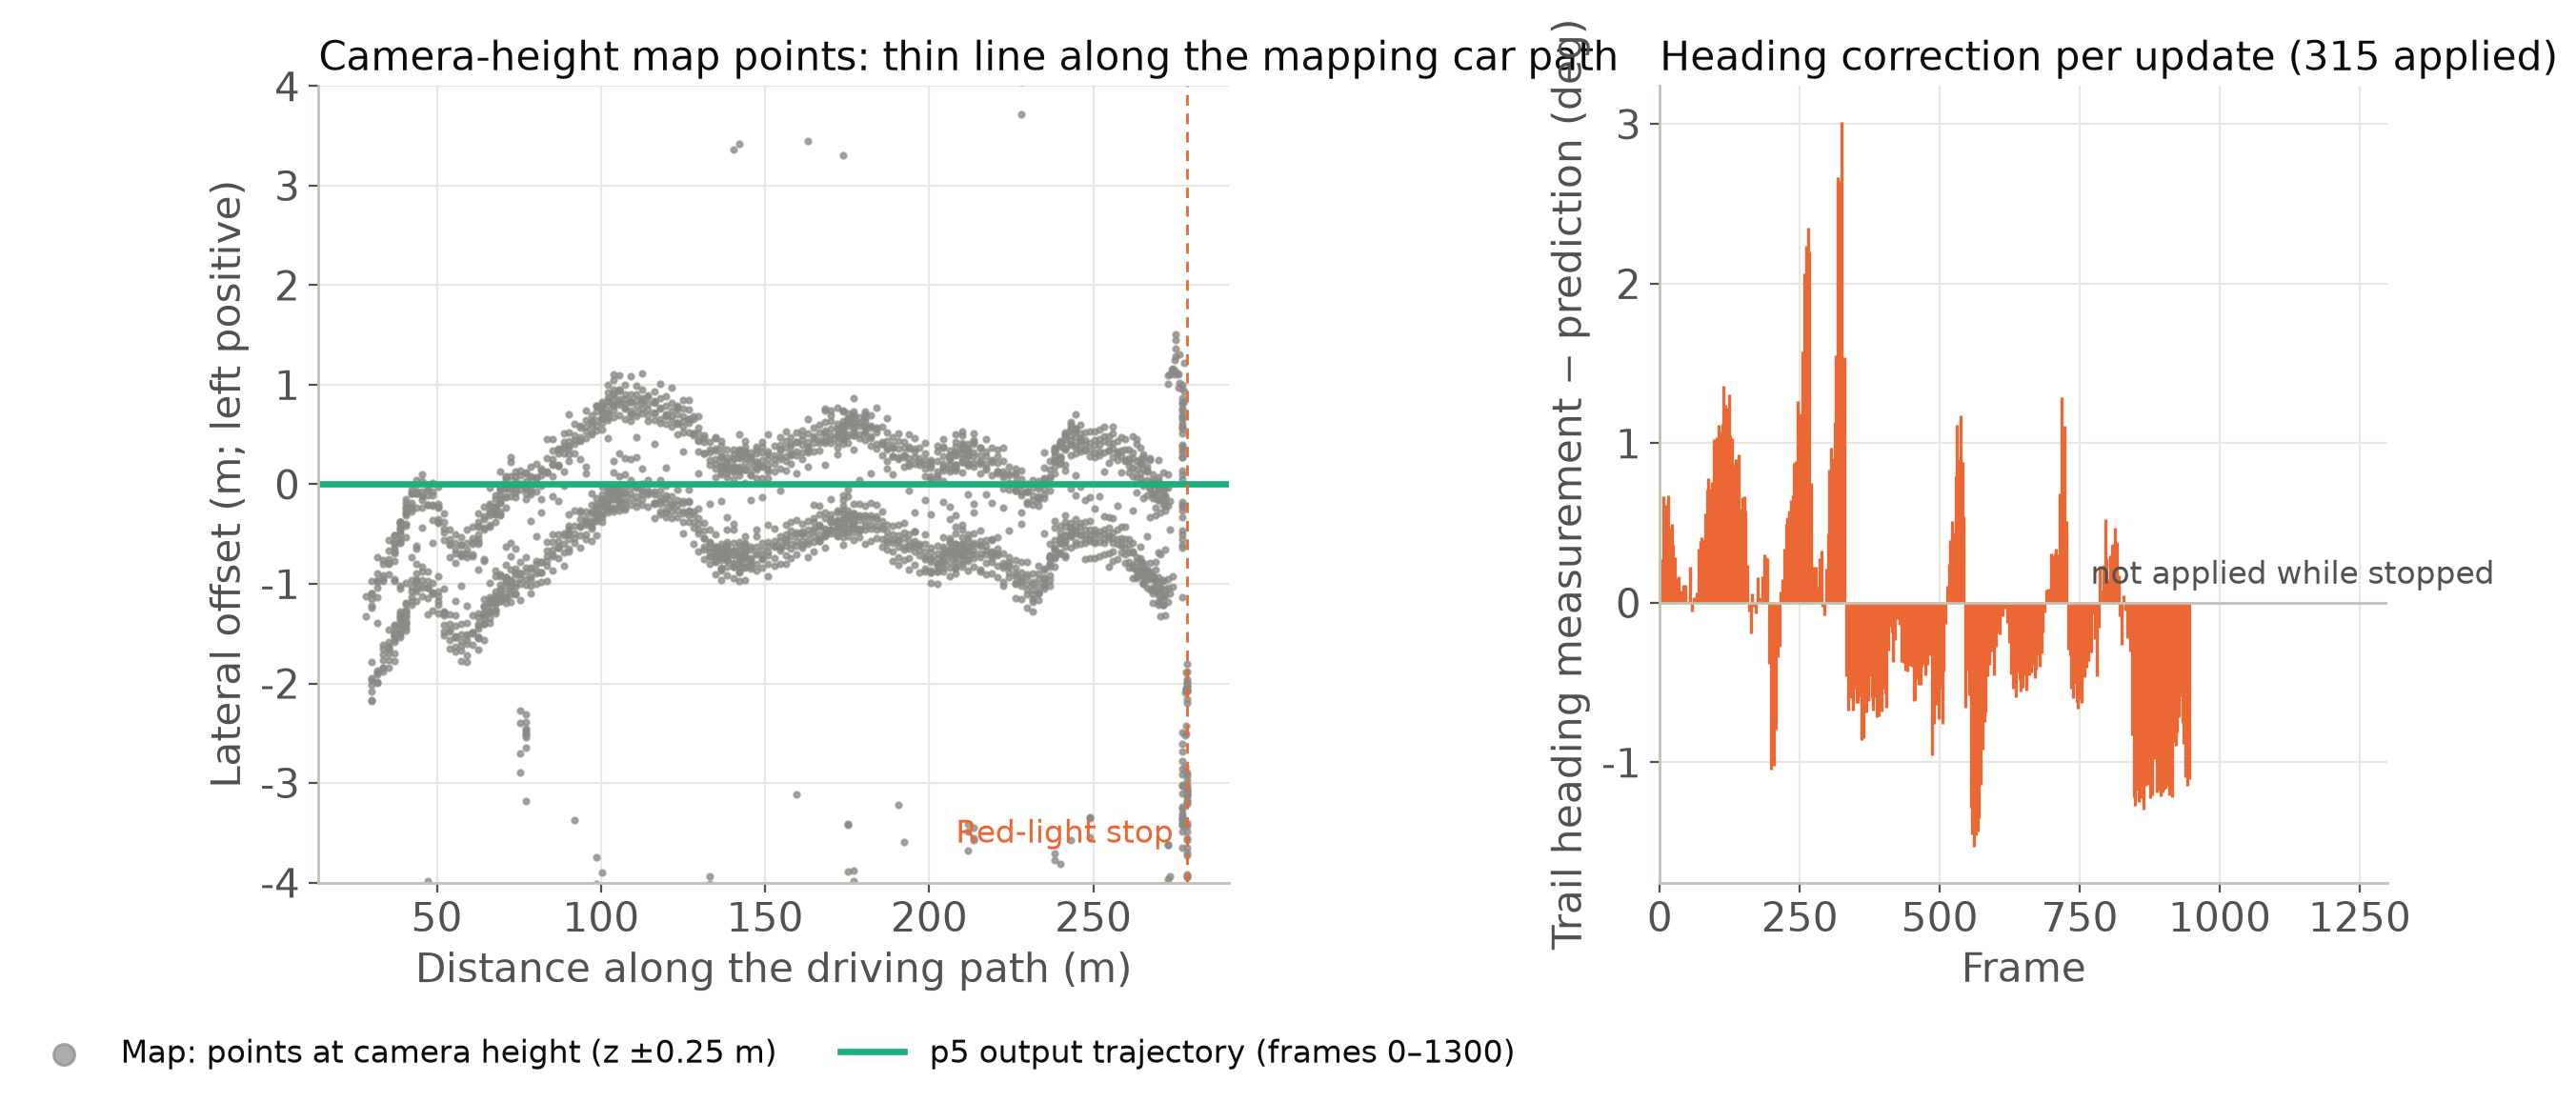
\includegraphics[width=\linewidth]{figures/fig07_trail_heading.png}
\caption{左：相機高度的地圖點沿建圖車軌跡形成細線（綠線為 \code{p5} 輸出）；
右：每次量測相對預測的航向修正量（停等時不量測）。}
\label{fig:trail}
\end{figure}

\textbf{做法}（\code{TrailHeading}）：每 3 幀、車輛非靜止且 NDT 收斂時，
\begin{enumerate}
  \item 取車體前後 12~m、左右 3~m、高度在位姿 $z\pm0.5$~m 內的子地圖點，做 2D PCA；
  \item 要求線夠細（短軸/長軸 $<0.25$）、夠長（$>6$~m）、至少 40 點；
  \item 線方向（模 180\dg）取與目前 yaw 最接近者，若相差超過 12\dg 則放棄（閘門）；
  \item 以其相對 yaw 的差 $\delta$ 作為 yaw 的純量量測，$\sigma=1.5$\dg，做卡爾曼更新（Joseph 形式）。
\end{enumerate}
靜止時不量測（yaw 本來就被凍結）。我們同時把 NDT 的 yaw 量測標準差由 2\dg{} 放寬為 4\dg，讓陀螺儀在 yaw 上更主導。

\textbf{離線驗證}（Track1/2，對 GNSS）：線方向與車頭夾角的中位數為 0.8\dg；
``線方向加 yaw 誤差'' 的 RMS 為 1.95\dg/2.10\dg，與 NDT 的 yaw 誤差（2.27\dg/3.03\dg）相當，且彼此獨立。

\textbf{效果（Track3）}：紅燈結束時的突然逆時針偏轉由 $+4.1$\dg 降到 $+0.5$\dg；
Kaggle \code{ba2} 2.01 $\to$ \code{bt1} 1.87 $\to$ \code{p5} 1.74（\code{p5} 為 $\sigma_{\psi}'=4$\dg、軌跡線 $\sigma=1.5$\dg、每 3 幀）。
public 區段（第 157--1257 幀）輸出減 IMU 姿態的平均偏差由 \code{bt1} 的 $+2.09$\dg 降到 $+1.34$\dg。
\textbf{限制}：軌跡線對起步時已長出的 700--1000 幀殘餘只修回約 0.3--1.2\dg；殘餘的根因（NDT 被單側結構拉偏）
本身沒有消除，只是被獨立的航向量測壓低。

\subsection{不採用的變體}
\begin{itemize}
  \item \textbf{停等時也量測軌跡線}（\code{b3}）：停等位置 yaw 被修到 $-1.1$\dg，Kaggle 反而由 1.87 變為 1.92（過修約 1.5--1.8\dg）。
  \item \textbf{軌跡線橫向推}（\code{l2}）：Kaggle 1.74$\to$1.84；Track1 發散；軌跡線的橫向位置不能當真值，方向才可靠。
  \item \textbf{左右不平衡降權}、\textbf{依左右選用 yaw 量測}：效果正負參半，不採用。
  \item \textbf{用地圖路面約束位姿 $z$}：轉彎太晚、轉彎後偏右，fitness 由 0.253 變差為 0.337。
  \item \textbf{固定前向倍率}（\code{ply_aniso_x}）：單幀診斷預期的改善在全長沒有重現。
\end{itemize}

%====================================================================
\section{問題 E：缺乏全域錨定——融入官方提供的 GNSS 先驗}\label{sec:E}

\textbf{說明}：Track1/2 的 bag 內含助教提供的 GNSS 位姿，官方文件明文允許使用。
這部分是對現成資料的\emph{融合}，不是我們的原創方法；以下說明融合的技術細節。
純相對估計（IMU 加 NDT）的誤差會隨時間累積，GNSS 提供全域的位置與航向錨點。

\subsection{讀取與因果性}
\code{GnssPrior} 讀取 bag 的 \code{/localizer_node/gnss_pose}（PoseStamped，約 4~Hz，影格間隔約 36~ms，
約每 7 幀有一筆），yaw 取自四元數 $\psi_g=2\,\mathrm{atan2}(q_z,q_w)$，並依時間排序。
每一幀\textbf{只取時間戳不晚於影格時間、且尚未使用過的最新一筆}（causal，每筆只用一次）；
若該筆比影格舊超過 600~ms 就丟棄。

\subsection{時間對齊與位置更新}
GNSS 樣本比影格早 $\Delta t$ 秒。為了讓位置量測對應影格時刻，以目前濾波器的速度 $v$ 與航向 $\psi$ 外推：
\begin{equation}
\mathbf z_{xy}=\mathbf g_{xy}+v\,\Delta t\begin{bmatrix}\cos\psi\\ \sin\psi\end{bmatrix},\qquad
\sigma=\sqrt{\sigma_{xy}^{2}+(0.3\,v\,\Delta t)^{2}},\quad \sigma_{xy}=0.7~\text{m}.
\end{equation}
第二項把外推本身的不確定度（以速度的 30\% 計）加進量測標準差。
接著對 $x,y$ 做卡爾曼更新：$H$ 選出前兩個狀態，$R=\sigma^2I_2$，
\[
K=PH^{\top}(HPH^{\top}+R)^{-1},\quad \mathbf x\leftarrow\mathbf x+K(\mathbf z_{xy}-H\mathbf x),\quad
P\leftarrow(I-KH)P(I-KH)^{\top}+KRK^{\top}\ \text{（Joseph 形式）}.
\]
因為位置與 yaw、速度等狀態有交叉協方差，位置更新同時會微調其餘狀態；更新後同步位姿的平移與 yaw。

\subsection{航向更新}
航向量測是純量更新：創新 $\delta=\mathrm{wrap}(\psi_g-\psi)$，標準差 $\sigma_{\psi}^{g}=2$\dg，
$K=P_{:,\psi}/(P_{\psi\psi}+\sigma_{\psi}^{g\,2})$，同樣用 Joseph 形式。
這個純量更新與軌跡線航向量測共用（第~\ref{sec:D} 節）。

\subsection{與其他量測的先後順序與例外}
每幀的順序為：IMU 預測 $\to$ NDT 融合量測更新 $\to$ GNSS 位置更新 $\to$ GNSS 航向更新 $\to$（Track3）軌跡線更新。
兩個例外：（1）第 0 幀不套用（此時由初始位姿搜尋或牆面先驗決定初值）；
（2）YawBank 運作期間不套用，因為各 yaw 假設各自獨立，GNSS 會偏袒某一假設。
GNSS 的位置與航向可以各自開關（\code{gnss_prior_use_xy}、\code{gnss_prior_use_yaw}），預設全關，逐 track 以 yaml 啟用。

\subsection{權重與消融}
$\sigma_{xy}=0.7$~m 與 $\sigma_{\psi}^{g}=2$\dg 為我們選定的權重（GNSS 本身雜訊約 0.7~m、固定偏移約 0.5~m）。
表~\ref{tab:gnss} 是 Kaggle public 的消融：位置資訊貢獻大部分改善；yaw 單獨使用幫助較小，
但對 Track2 靜止起步的 yaw 有效（前 300 幀的 yaw 平均被拉動約 5\dg）。
由於 GNSS 同時是本地評估的參考，啟用 GNSS 的版本對 GNSS 的本地 $E$ 是循環的，只引用 Kaggle 分數。

\begin{table}[H]
\centering\small
\caption{GNSS 先驗消融（Kaggle public）}\label{tab:gnss}
\begin{tabular}{@{}lcccc@{}}
\toprule
 & 無 GNSS & 只用 xy & 只用 yaw & xy + yaw\\
\midrule
Track1 & 1.52 & 1.17 & 1.47 & \textbf{1.13}\\
Track2 & 1.46 & 0.78 & 1.38 & \textbf{0.77}\\
\bottomrule
\end{tabular}
\end{table}

%====================================================================
\section{結果}

\subsection{Track3 的分數演進}
\begin{figure}[H]
\centering
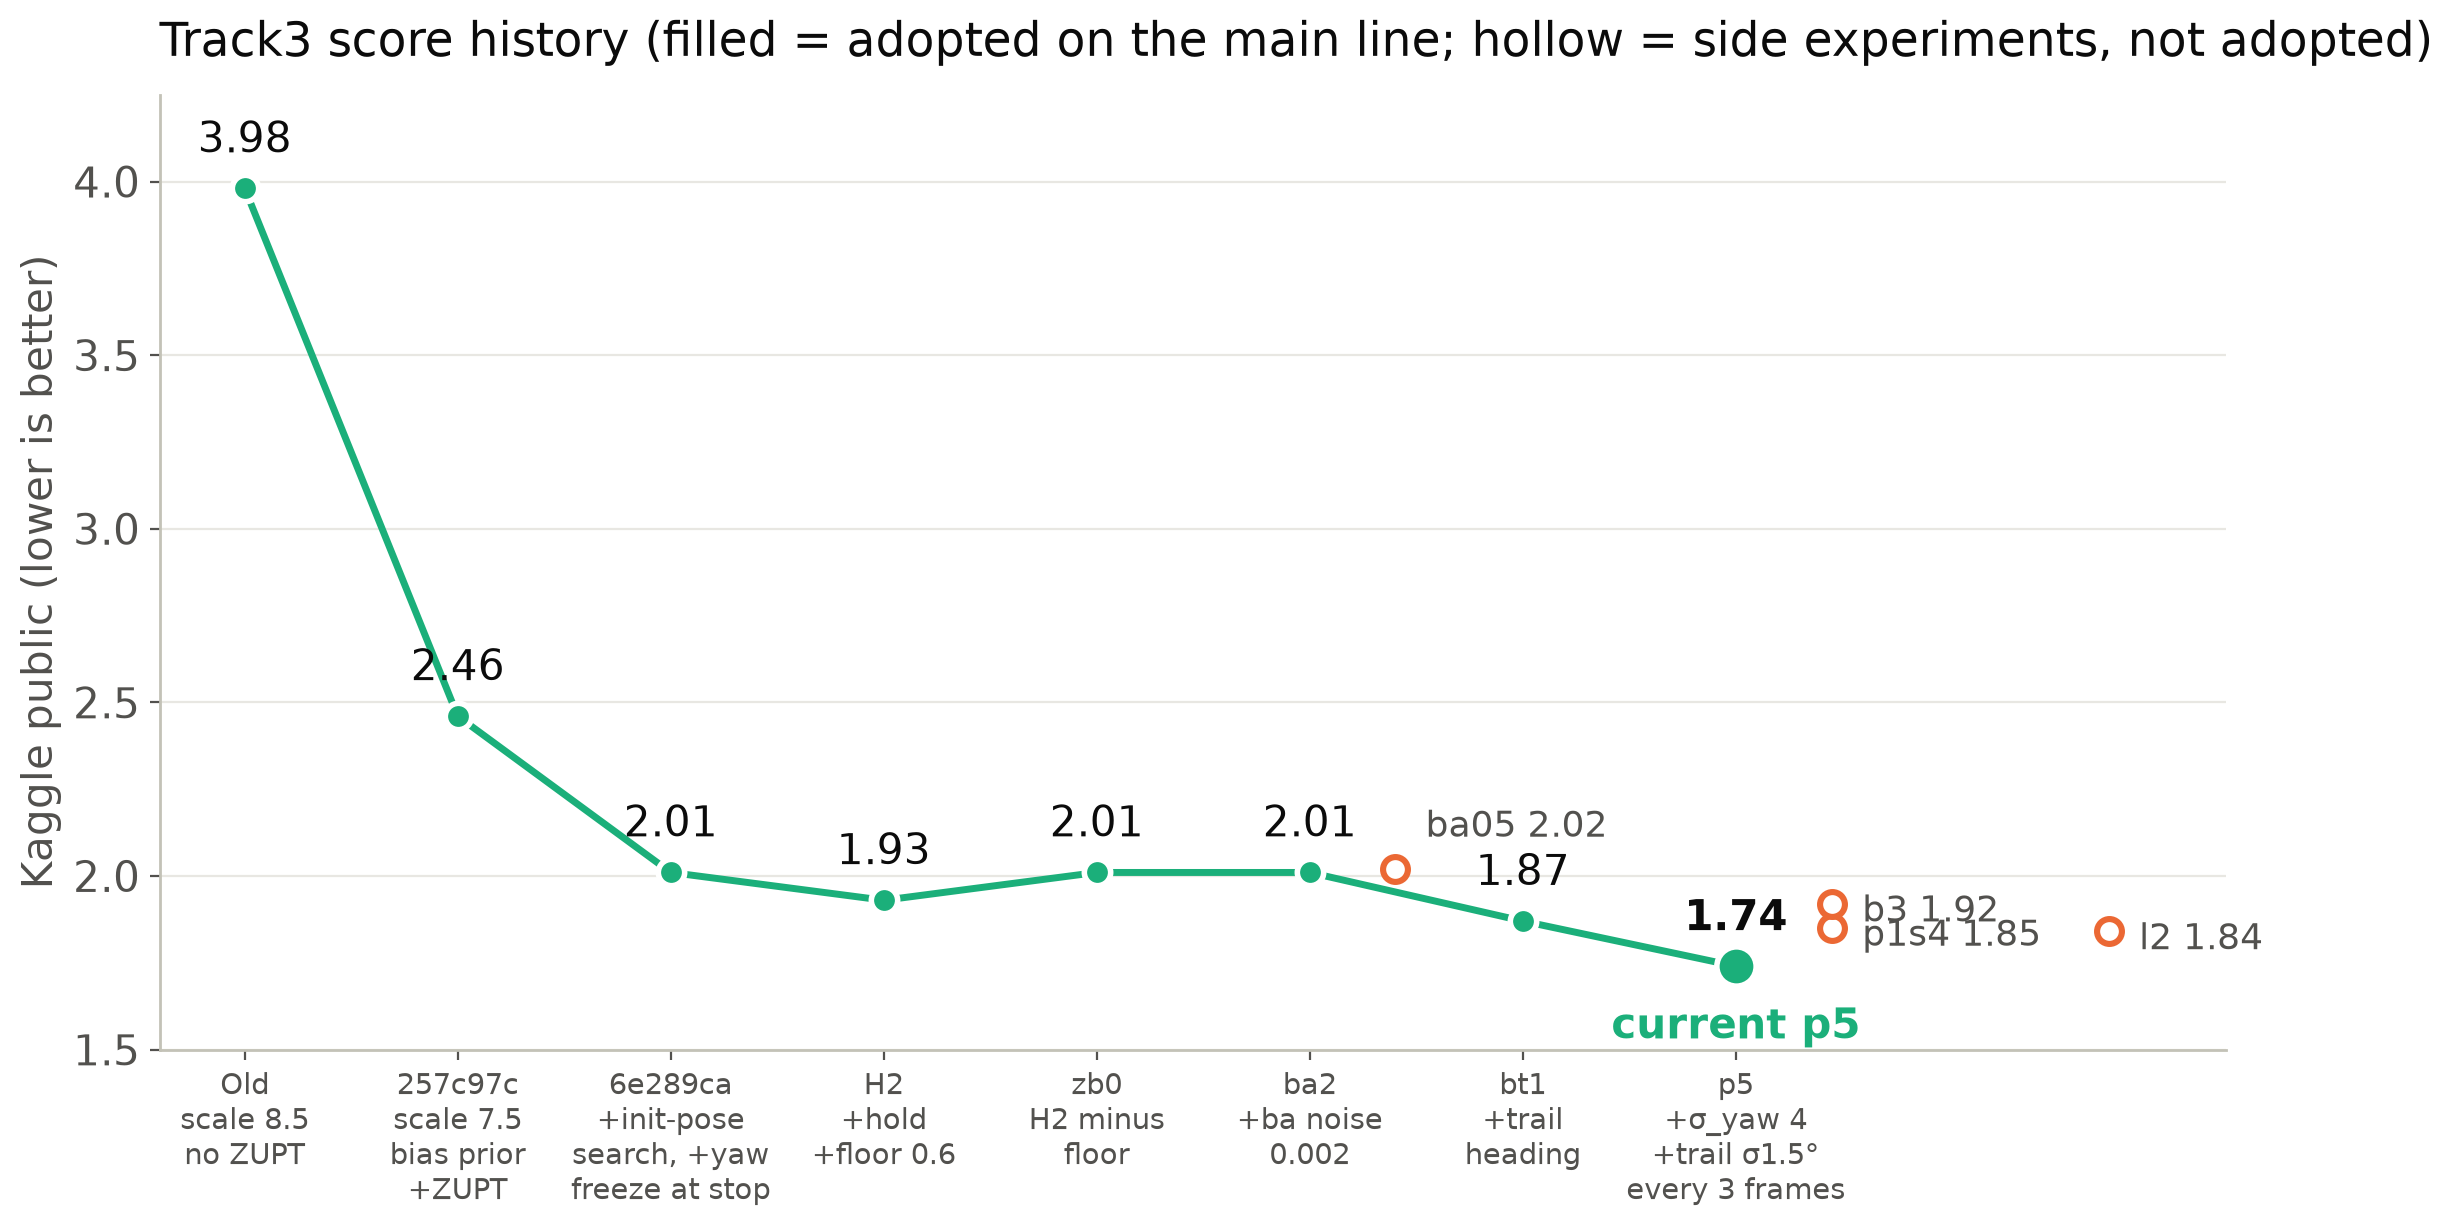
\includegraphics[width=\linewidth]{figures/fig08_track3_progress.png}
\caption{Track3 Kaggle public 分數演進。實心為主線採用的版本，空心為支線試驗（\code{ba05}、\code{b3}、\code{p1s4}、\code{l2}）、未採用。}
\label{fig:t3}
\end{figure}

\subsection{各 track 版本對照（Kaggle public）}
\begin{table}[H]
\centering\small
\caption{各版本相對父版本的新增項目與 Kaggle 分數}\label{tab:versions}
\begin{tabularx}{\linewidth}{@{}llYc@{}}
\toprule
Track & 版本 & 新增 & Kaggle\\
\midrule
T1 & \code{5597dfe} & 共同基礎 & 1.56\\
T1 & \code{047f72a} & +floor 0.6、搜 xy 格 & 1.62（退步）\\
T1 & \code{rhp1s4} & 只搜 yaw、$\sigma_{\psi}'=4$\dg & 1.52\\
T1 & \textbf{\code{gb}} & +GNSS xy+yaw & \textbf{1.13}\\
\midrule
T2 & \code{rhp2} & 收斂版+牆面先驗、$\sigma_{\psi}'=4$\dg & 1.46\\
T2 & \textbf{\code{g2b}} & +GNSS xy+yaw & \textbf{0.77}\\
\midrule
T3 & 舊版 & scale 8.5、無 ZUPT & 3.98\\
T3 & \code{257c97c} & scale 7.5+零偏先驗+ZUPT & 2.46\\
T3 & \code{6e289ca} & +初始位姿搜尋+靜止凍結 yaw & 2.01\\
T3 & H2（\code{f81f508}） & +hold+floor 0.6（floor 後來移除） & 1.93\\
T3 & \code{bt1} & +$b_a$ 雜訊 0.002+軌跡線 & 1.87\\
T3 & \code{p1s4} & \code{bt1}+$\sigma_{\psi}'=4$\dg & 1.85\\
T3 & \textbf{\code{p5}} & +$\sigma_{\psi}'=4$\dg+軌跡線 $\sigma=1.5$\dg、每 3 幀 & \textbf{1.74}（private 1.36）\\
\bottomrule
\end{tabularx}
\end{table}

\subsection{評估的限制}
\begin{itemize}
  \item GNSS 只有約 4~Hz、雜訊約 0.7~m、固定偏移約 0.5~m，分不出 0.05--0.17 的差距與逐幀抖動，
        所以調參時同時看平滑度（位置二階差）與 Kaggle。
  \item Track3 沒有真值也沒有 GNSS；public 只評約第 157--1257 幀，轉彎（約 2400--2800 幀）落在 private，
        只能靠 RViz 人工目視判斷。
\end{itemize}

%====================================================================
\section{尚未解決的問題}
Track3 public 1.74 仍高於 public baseline 1.29。誤差預算（推論，Track3 無真值）：位置 RMSE 約 1.2~m，
加上 $0.2\times$ yaw RMS（約 2.5\dg）；橫向偏差（0.3--0.5~m）僅貢獻 0.04--0.1，停等位置縱向偏差不超過 0.5~m；
剩下的誤差\textbf{很可能}主要在行駛段的縱向（NDT 退化方向）與 yaw。單幀診斷顯示尺度每差 1 單位，
縱向最佳位置移動約 1.7~m，可能與尺度耦合，但全長未驗證。另外，轉彎後位姿 $z$ 偏高約 0.5--0.9~m、
pitch 鼻朝下，只確認了現象，尚未解決。
未做的方向：估計 NDT yaw 量測相對軌跡線方向的緩變偏差並從量測中扣除；轉彎段的縱向約束。

%====================================================================
\section{Workload Distribution}
\begin{table}[H]
\centering\small
\begin{tabularx}{\linewidth}{@{}llYc@{}}
\toprule
成員 & 學號 & 負責項目 & 貢獻比例\\
\midrule
王修呈 & a151527 & 初始環境、初版程式、開發方向與研究計畫、實驗結果分析與提出改進方向 & 100\%\\
Claude & --- & 撰寫程式與執行實驗 & 100\%\\
\bottomrule
\end{tabularx}
\end{table}

%====================================================================
\section{Others}

\subsection{重現方式}
細節見 \code{README.md}。以 Track1 為例：
\begin{lstlisting}[language=bash]
docker compose up -d && docker exec -it mid1_container bash
cd /root/midterm
colcon build --packages-select localization --cmake-args -DCMAKE_BUILD_TYPE=Release
source install/setup.bash
ros2 launch localization map_modified.launch.py data_path:=/root/data/Track1 voxel_leaf_size:=1.0
ros2 launch localization localization.launch.py data_path:=/root/data/Track1 save_file:=Track1_result.txt
python3 src/localization/processing_codes/txt_to_idx_x_y_yaw.py \
    src/localization/result/Track1_result.txt src/localization/result/result_1.csv
\end{lstlisting}
Track2/3 同理，將 \code{data_path} 換成對應目錄即可；參數檔依目錄名稱自動選用。

\subsection{三份 yaml 的刻意差異}
\begin{itemize}
  \item \code{ply_scale}：8.5/8.7/7.5。
  \item Track1：初始位姿搜尋只搜 yaw；開啟 \code{gnss_prior_*}。
  \item Track2：關閉初始位姿搜尋；開啟牆面方向先驗（\code{road_heading_*}）、YawBank（\code{yaw_bank_*}）、
        $b_a$ 偽量測、釘住 $\beta$；開啟 \code{gnss_prior_*}。
  \item Track3：初始位姿搜尋含 xy 格；開啟軌跡線航向量測（\code{trail_heading_*}）。
\end{itemize}
可用 \code{tools/diff_params.py} 檢查三份 yaml 的差異。

\end{document}
